\documentclass{article}
\usepackage{graphicx}
\usepackage{amsmath}
\usepackage{tikz}
\usetikzlibrary{intersections}
\usetikzlibrary{arrows.meta,calc}
\usetikzlibrary{angles,quotes}
\usepackage{placeins}

\begin{document}

\section{Design Calculations}

\subsection{Given Requirements}

\begin{itemize}
\item Maximum mass: $m_{\max} = 2000\text{g} = 2.0\text{kg}$
\item Nominal speed: $v = 350\text{mm/s} = 0.35\text{m/s}$
\item Footprint: circular, diameter $D = 50\text{-}60\text{cm}$
\item Stair height: $h = 2.5 \text{cm}  = 0.025\text{m}$
\item Minimum runtime: $t = 15 \text{min} = 0.25 \text{h}$
\item PCB reserved volume: $150 \times 150 \times 100\text{mm}^3$
\item Visual feedback: $\geq 300$ lumen
\end{itemize}

For the design, a footprint diameter of $D = 550\text{mm}$ is selected.
\[
R_{\text{robot}} = \frac{D}{2} = 275\,\text{mm}
\]

All robot components must lie within this radius.

\subsection{Climbing Force Derivation}

\begin{center}
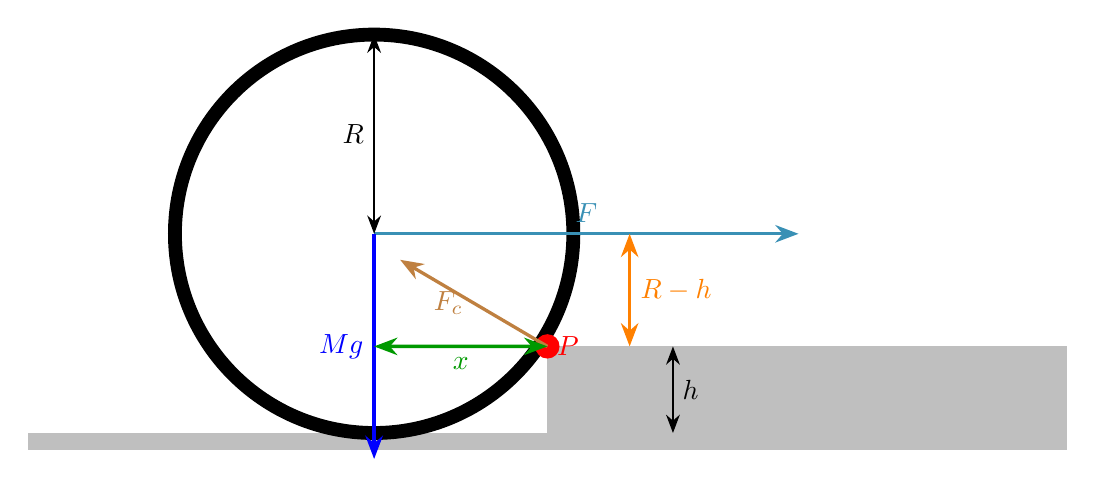
\begin{tikzpicture}[scale=1.1, >=Stealth]
    % Parameters
    \def\R{2.3}
    \def\hub{0.45}
    \def\stepH{1.0}
    \def\cx{0}
    \def\cy{\R}

    % Ground and step
    \fill[black!25] (-4,-0.2) rectangle (8,0);
    \fill[black!25] (2,0) rectangle (8,\stepH);

    % Wheel outer tire
    \draw[line width=5pt, black] (\cx,\cy) circle (\R);

    % Contact - pivot point at step corner
    \coordinate (P) at (2,\stepH);
    \fill[red] (P) circle (4pt) node[right] {$P$};

    % Horizontal force arrow F
    \draw[very thick, cyan!70!black, ->]
        (\cx,\cy) -- (4.9,\cy) node[midway, above] {$F$};

    % Weight Mg
    \draw[very thick, blue, ->]
        (\cx,\cy) -- (\cx,-0.3) node[midway, left] {$Mg$};

    % Contact force from center to pivot
    \draw[very thick, brown, <-] (\cx+0.3,\cy-0.3) -- (P) node[midway, left] {$F_c$};
    % Green horizontal arm
    \draw[<->, very thick, green!60!black] (\cx,\stepH) -- (P) node[midway, below] {$x$};

    % Small orange vertical near step edge
    \draw[<->, very thick, orange] (2.95,\stepH) -- (2.95,\cy) node[midway, right] {$R-h$};

    % Radius label R on left
    \draw[<->, thick] (\cx,\cy) -- (0,\R*2) node[midway, left] {$R$};

    % Step height h
    \draw[<->, thick] (3.45,0) -- (3.45,\stepH);
    \node[right] at (3.45,{\stepH/2}) {$h$};
\end{tikzpicture}
\end{center}

Torque is a product of force and its perpendicular distance from the pivot:
\[
\tau = rF\sin\theta = F r_{\perp}
\]

At the moment when the wheel just starts to climb the step, the wheel rotates about the corner of the step, so we take torques about this pivot point $P$.

The contact force $F_c$ at the pivot does not create any torque, because its line of action passes through the pivot:
\[
\tau_{\text{pivot}} = 0
\]

The applied horizontal force $F$ acts at the wheel center. Its lever arm with respect to the pivot is the vertical distance $R-h$. Therefore its torque is
\[
\tau_F = F(R-h)
\]

The weight \(Mg\) acts vertically downward through the wheel center. Its lever arm is the horizontal distance \(x\) between the wheel center and the pivot.

From the right triangle:
\[
x = \sqrt{R^2 - (R-h)^2}
\]

Simplifying:
\[
x = \sqrt{R^2 - (R^2 - 2Rh + h^2)}
\]
\[
x = \sqrt{2Rh - h^2}
\]

So the torque due to gravity is
\[
\tau_{Mg} = Mg \sqrt{2Rh - h^2}
\]

At the threshold of climbing, the torques are balanced:
\[
\tau_F = \tau_{Mg}
\]

Hence
\[
F(R-h) = Mg \sqrt{2Rh - h^2}
\]

Solving for \(F\), we obtain

\begin{equation}
F = \frac{Mg \sqrt{2Rh - h^2}}{R - h}
\label{eq:climbing_force}
\end{equation}

\[
h \to R \quad \Rightarrow \quad F \to \infty
\]


\subsection{Wheel Radius Selection}

From the previous analysis, it follows that the wheel radius must satisfy $R>h$.

Here, we choose

\[
\boxed{R= 1.7h=42.5\ \text{mm}}
\]

This corresponds to a wheel diameter of

\[
\boxed{d = 2R = 85\ \text{mm}}
\]


\subsection{Calculation Climbing Force}

Assuming an even distribution of mass across four wheels:

\[
m_{\text{wheel}} = \frac{m}{4} = \frac{2.0}{4} = 0.5\ \text{kg}
\]

Using the previously derived expression \eqref{eq:climbing_force}, the corresponding climbing force per wheel is:

\[
F = \frac{m_{\text{wheel}}g\sqrt{2Rh - h^2}}{R - h}
\]

Substituting numerical values:

\[
F = \frac{(0.5)(9.81)\sqrt{2(0.0425)(0.025) - (0.025)^2}}{0.0425 - 0.025}
\]

\[
\boxed{F \approx 10.9\ \text{N}}
\]

\subsection{Required Wheel Torque}

The torque required at the wheel is:

\[
\tau = F R
\]

\[
\tau = 10.9 \cdot 0.0425 \approx 0.461\ \text{N\,m}
\]

\[
\boxed{\tau \approx 0.46\ \text{N\,m}}
\]

To account for uncertainties such as uneven load distribution, friction, and dynamic effects, a safety factor is applied:

\[
\tau_{\text{design}} = S \cdot \tau
\]

Using \(S=2\):

\[
\tau_{\text{design}} = 2 \cdot 0.46 = 0.92\ \text{N\,m}
\]

\[
\boxed{\tau_{\text{design}} \approx 0.92\ \text{N\,m}}
\]

\subsection{Wheel Angular Velocity}

The relationship between linear velocity and angular velocity is given by

\[
v = \omega R
\]

Solving for \(\omega\):

\[
\omega = \frac{v}{R}
\]

Substituting the nominal velocity \(v = 0.35\ \text{m/s}\) and \(R = 0.0425\ \text{m}\):

\[
\omega = \frac{0.35}{0.0425} \approx 8.24\ \text{rad/s}
\]

Converting to revolutions per minute:

\[
n = \frac{60\omega}{2\pi}
\]

\[
n = \frac{60 \cdot 8.24}{2\pi} \approx 78.7\ \text{RPM}
\]

\[
\boxed{n \approx 79\ \text{RPM}}
\]

\subsection{LED Brightness Verification}

To satisfy the requirement of at least \(300\,\text{lumen}\), high-power LEDs are used, 1\,W white LED provides:
\[
\Phi_{\text{LED}} \approx 100\,\text{lumen}
\]
To meet the requirement with a safety margin, four LEDs are used:
\[
\Phi_{\text{total}} = 4 \cdot 100 = 400\,\text{lumen} \geq 300\,\text{lumen} \quad
\]

Each LED consumes \(P_{\text{LED}} = 1\,\text{W}\), giving a total optical power of:
\[
\boxed{P_{\text{LED,total}} = 4\,\text{W}}
\]

High-power LEDs require current control and cannot be connected directly to a voltage source.
With four LEDs connected in series, the total forward voltage equals the supply voltage:
\[
V_{\text{LED,total}} = 4 \cdot 3\,\text{V} = 12\,\text{V} = V_{\text{supply}}
\]
This leaves no room for a series resistor:
\[
R = \frac{V_{\text{supply}} - V_{\text{LED,total}}}{I} = \frac{12 - 12}{0.3} = 0\,\Omega
\]
Therefore, a single resistor current limiting approach is not working here.

But we can arrange four LEDs in parallel wires, each containing two LEDs in series.
Each wire is supplied from 12\,V with a current-limiting resistor:
\[
R = \frac{V_{\text{supply}} - 2\,V_{\text{LED}}}{I} = \frac{12 - 6}{0.3} = 20\,\Omega
\]
The power on each resistor is:
\[
P_R = I^2 \cdot R = (0.3)^2 \times 20 = 1.8\,\text{W}
\]
A resistor with a power rating of at least \(2\,\text{W}\) is selected to ensure safe operation.


\subsection{Motor Requirements}

Each of the four wheels is driven by an individual motor. Therefore, for the maximum possible mass {2 kg} each motor must satisfy:

\[
\boxed{n \approx 79\ \text{RPM}}
\]

\[
\boxed{\tau \ge 0.92\ \text{N\,m}}
\]

\subsection{Estimated Mechanical Power}

The mechanical power per wheel is given by:

\[
P = \tau_{\text{design}} \omega
\]

\[
P = 0.92 \cdot 8.24 \approx 7.58\ \text{W}
\]

Thus, each motor must provide at least:

\[
\boxed{P \approx 7.6\ \text{W per motor}}
\]


\subsection{Total Power Computation}

The electrical power consumption of each component is calculated using

\[
P = U \cdot I
\]

A DC Geared-Down Motor 37Dx70L 10 W motor is selected for each wheel.

\[
P_{\text{motor}} = 10\ \text{W}
\]


For four motors:

\[
P_{\text{motors,total}} = 4 \cdot 10 = 40\ \text{W}
\]

Taking into account efficiency

\[
\eta = 0.7
\]

the required electrical power becomes

\[
P_{\text{elec}} = \frac{40}{0.7} = 57.14\ \text{W}
\]


ESP32 (Microcontroller):
it processes sensor data and controls the motors, enabling tasks such as navigation, line tracking, and obstacle avoidance.

\[
P_{\text{ESP32}} = 5 \cdot 0.16 = 0.80\ \text{W}
\]

HC-SR04 (Ultrasonic Sensor):
it is used to measure the distance to obstacles. It allows the robot to detect objects in front of it and avoid collisions.

\[
P_{\text{HC-SR04}} = 5 \cdot 0.015 = 0.075\ \text{W}
\]

LEDs:
they are used for visual feedback, such as indicating the robot’s status or improving visibility in low-light conditions. We use 4 LEDS.

\[
P_{\text{LED,total}} = 4.0\ \text{W}
\]

Resistors (LED current limiting):

\[
P_{R,\text{total}} = 2 \cdot 1.8 = 3.6\ \text{W}
\]

LM2596 Buck Converter:
it is a step-down (DC-DC) converter used to reduce the battery voltage (12V) to a lower voltage (5V) required by the ESP32 and sensors.

\[
P_{\text{buck}} = 12 \cdot 0.005 = 0.06\ \text{W}
\]

Infrared Line Tracking Sensor (TCRT5000):

it is used for line tracking. It detects the contrast between a dark line and a surface by measuring reflected infrared light, allowing the robot to follow a predefined path.

\[
P_{\text{IR}} = 5 \cdot 0.05 = 0.25\ \text{W}
\]


Summing all contributions:

\[
P_{\text{total}} =
57.14 + 0.80 + 0.075 + 4.0 + 3.6 + 0.06+0.25
\]

\[
P_{\text{total}} = 65.925\ \text{W}
\]

\[
\boxed{P_{\text{total}} \approx 65.93\ \text{W}}
\]

\begin{table}[h!]
\centering
\begin{tabular}{|l|c|c|c|c|}
\hline
\textbf{Component} & \textbf{Voltage(V)} & \textbf{Current(A)} & \textbf{Quantity} & \textbf{Power (W)} \\
\hline
JGB37 Gear Motor & 12 & 1.19 & 4 & 57.14 \\
ESP32 Development Board & 5 & 0.16 & 1 & 0.80 \\
HC-SR04 Ultrasonic Sensor & 5 & 0.015 & 1 & 0.075 \\
TCRT5000 Infrared Line Tracking Sensor & 5 & 0.05 & 1 & 0.25 \\
1W LED Diode & 3 & 0.3 & 4 & 4.0 \\
LM2596 Buck Converter & 12 & 0.005 & 1 & 0.06 \\
\hline
\textbf{Total Power} &  &  &  & \textbf{65.93} \\
\hline
\end{tabular}
\label{tab:power_consumption}
\end{table}

\subsection{Battery Sizing }

The required operating time is

\[
t = 0.25h
\]

Thus, the required battery energy is

\[
E = P_{\text{total}} \cdot t
\]

\[
E = 65.93 \cdot 0.25 = 16.48\ \text{Wh}
\]

\[
\boxed{E=16.48\ \text{Wh}}
\]

Assuming

\[
V = 12\ \text{V}
\]

the minimum battery capacity is

\[
C = \frac{E}{V}
\]

\[
C = \frac{16.48}{12} = 1.37\ \text{Ah}
\]

\[
\boxed{C_{\min} = 1.37\ \text{Ah}}
\]
\subsection{Clearance Height of the Robot Body}

To verify whether the bottom of the robot collides with the step during climbing, a geometric clearance analysis is performed.


%Figure 1: before climbing
\begin{figure}[h!]
\centering
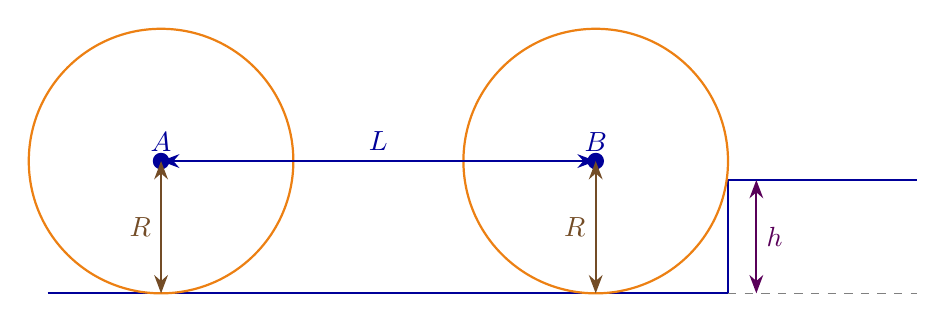
\begin{tikzpicture}[scale=1.2, >=Stealth]

\def\R{1.4}
\def\stepH{1.2}
\def\xA{0}
\def\xB{4.6}
\def\yC{\R}

\draw[thick, blue!60!black] (-1.2,0) -- (6,0);
\draw[thick, blue!60!black] (6,0) -- (6,\stepH);
\draw[thick, blue!60!black] (6,\stepH) -- (8,\stepH);

\draw[dashed, gray] (6,0) -- (8,0);

\draw[thick, orange!70!brown] (\xA,\R) circle (\R);
\draw[thick, orange!70!brown] (\xB,\R) circle (\R);

\fill[blue!60!black] (\xA,\yC) circle (2.5pt) node[above] {$A$};
\fill[blue!60!black] (\xB,\yC) circle (2.5pt) node[above] {$B$};

\draw[<->, thick, blue!60!black] (\xA,\yC) -- (\xB,\yC)
node[above, midway] {$L$};

\draw[<->, thick, brown!60!black] (\xA,0) -- (\xA,\R)
node[left, midway] {$R$};

\draw[<->, thick, brown!60!black] (\xB,0) -- (\xB,\R)
node[left, midway] {$R$};

\draw[<->, thick, violet!70!black] (6.3,0) -- (6.3,\stepH)
node[right, midway]{$h$};

\end{tikzpicture}
\caption{Wheels approaching a step}
\end{figure}

For this analysis, it is assumed that the distance from the robot body to the ground is equal to the wheel radius R. The goal is to check whether the lower side of the robot body passes above the edge of the step.

%Figure 2: One wheel on a stair
\begin{figure}[htbp]
\centering
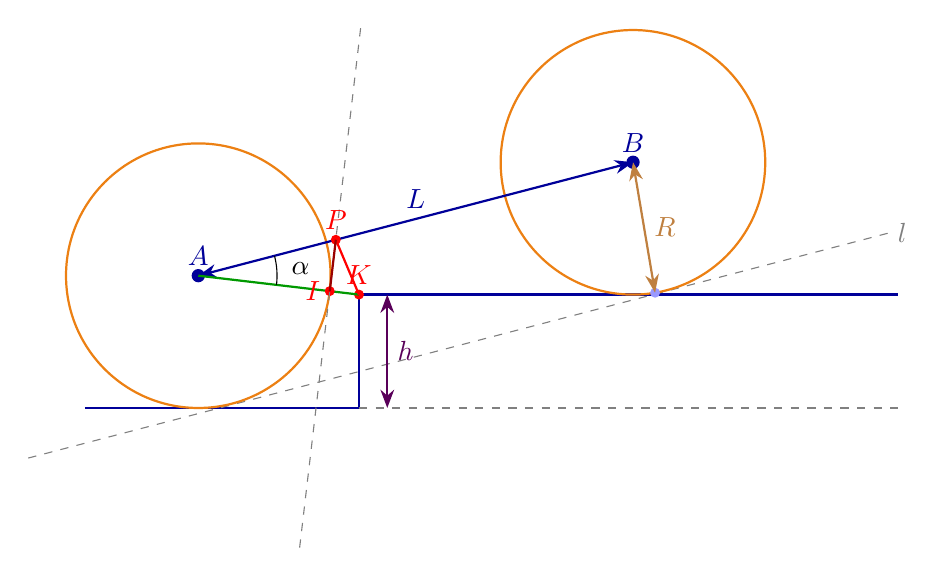
\begin{tikzpicture}[scale=1.2, >=Stealth]

\def\R{1.4}
\def\stepH{1.2}
\def\xA{0}
\def\yC{\R}
\def\xB{4.6}
\def\yB{\R+\stepH}

\coordinate (A) at (\xA,\R);
\coordinate (P) at (2.2,1.85);
\coordinate (B) at (\xB,\yB);
\coordinate (K) at (1.7, \stepH);

\fill[blue!60!black] (A) circle (2pt) node[above] {$A$};
\fill[blue!60!black] (B) circle (2pt) node[above] {$B$};

\draw[thick, blue!60!black] (-1.2,0) -- (1.7,0);
\draw[thick, blue!60!black] (1.7,0) -- (1.7,\stepH);
\draw[thick, blue!60!black] (1.7,\stepH) -- (7.4,\stepH);

\draw[dashed, gray] (1.7,0) -- (7.4,0);
\draw[dashed, gray, name path=l] (-1.8,-0.53) -- (7.3,1.85)
node[above, right] {$l$};

\draw[thick, orange!70!brown] (0,\R) circle (\R);
\draw[thick, orange!70!brown] (\xB,\yB) circle (\R);

\draw[<->, thick, blue!60!black] (A) -- (B)
node[above, midway] {$L$};

\fill[red] (K) circle (1.5pt) node[above] {$K$};

\draw[thick, green!60!black] (K) -- (A);

\path[name path=circleA] (A) circle (\R);
\path[name path=greenLine] (K) -- (A);
\path[name intersections={of=circleA and greenLine, by=I}];

\fill[red] (I) circle (1.5pt) node[above, left] {$I$};

\path[name path=AB] (A) -- (B);

\draw[dashed, gray, name path=tangent]
  ($(I)!-2!90:(A)$) -- ($(I)!2!90:(A)$);

\path[name intersections={of=tangent and AB, by=P}];
\fill[red] (P) circle (1.5pt) node[above] {$P$};

\path[name path=l] (-1.8,-0.53) -- (7.3,1.87);
\path[name path=circleB] (B) circle (\R);

\path[name intersections={of=l and circleB, by={J1,J2}}];

\fill[blue!40!white] (J1) circle (1.5pt);

\draw[<->, brown, thick] (J1) -- (B)
node [right, midway] {$R$};

\draw[red, thick] (K) -- (P);
\draw[red!60!black, thick] (I) -- (P);

\draw pic[
  draw=black,
  "$\alpha$",
  angle radius=10mm,
  angle eccentricity=1.3
] {angle=K--A--B};

\draw[<->, thick, violet!70!black] (2,0) -- (2,\stepH)
node[right, midway]  {$h$};

\end{tikzpicture}
\caption{Configuration during step climbing}
\end{figure}
\FloatBarrier
In the initial position, the robot approaches the step on a horizontal surface.  
In the critical configuration, the front wheel has already passed the step, and the robot is just about to lift the rear wheel.  
At this moment, the edge of the step, denoted by \(K\), is the critical point that could collide with the robot body.

A perpendicular is dropped from point \(K\) onto the line \(AB\), defining point \(P\).
From point \(P\), a tangent is drawn to the rear wheel, touching the wheel at point \(I\).
The segment \(PK\) represents the clearance between the robot body and the step edge.


For safe climbing, the condition is:

\[
\boxed{PK > 0}
\]

\subsubsection{Step 1: Inclination angle}


From the first triangle:

\[
\sin\alpha = \frac{h}{L}
\]

\[
\alpha = \arcsin\left(\frac{h}{L}\right)
\]

%Triangle 1
\begin{figure}[htbp]
\centering
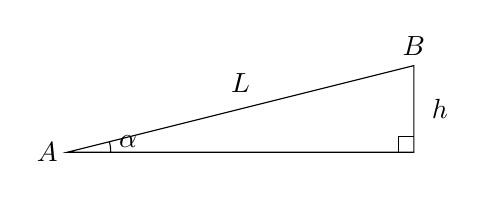
\begin{tikzpicture}[scale=1.1, >=Stealth]

\coordinate (A) at (0,0);
\coordinate (B) at (4,1);
\coordinate (C) at (4,0);

\draw (A) -- (B) -- (C) -- cycle;

\node[above, left] at (A) {$A$};
\node[above] at (B) {$B$};

\draw (A) ++(0.5,0) arc (0:14:0.5) node [right] {$\alpha$};
\draw pic [draw, angle radius=2mm] {right angle = A--C--B};

\node at (2,0.8) {$L$};
\node at (4.3,0.5) {$h$};

\end{tikzpicture}
\caption{Inclination angle of the robot}
\end{figure}

\FloatBarrier
\subsubsection{Step 2: Length \(AP\)}

From the second triangle:

\[
\cos\alpha = \frac{R}{AP}
\quad \Rightarrow \quad
AP = \frac{R}{\cos\alpha}
\]

%Triangle 2
\begin{figure}[h!]
\centering
\begin{tikzpicture}[scale=1.1, >=Stealth]

\coordinate (A) at (0,0);
\coordinate (P) at (4,1);
\coordinate (I) at (4,0);

\draw (A) -- (P) -- (I) -- cycle;

\node[left] at (A) {$A$};
\node[above] at (P) {$P$};
\node[right] at (I) {$I$};

\draw (A) ++(0.5,0) arc (0:14:0.5) node [right] {$\alpha$};
\draw pic [draw, angle radius=2mm] {right angle = A--C--B};

\node at (2,-0.3) {$R$};

\end{tikzpicture}
\caption{Triangle used to derive $AP$}
\end{figure}

\FloatBarrier

\subsubsection{Step 3: Clearance \(PK\)}

From the third triangle:

\[
\tan\alpha = \frac{PK}{AP}
\quad \Rightarrow \quad
PK = AP \tan\alpha
\]

Substituting:

\[
PK = \frac{R}{\cos\alpha} \tan\alpha
\]

\[
\boxed{
PK = \frac{R\tan\alpha}{\cos\alpha}
}
\]


%Triangle 3
\begin{figure}[h!]
\centering
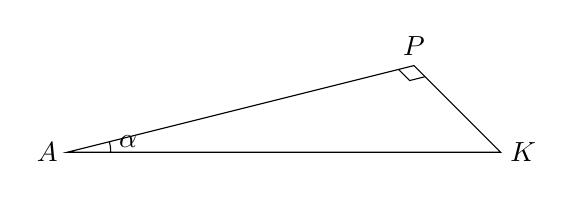
\begin{tikzpicture}[scale=1.1, >=Stealth]

\coordinate (A) at (0,0);
\coordinate (P) at (4,1);
\coordinate (K) at (5,0);

\draw (A) -- (P) -- (K) -- cycle;

\node[left] at (A) {$A$};
\node[above] at (P) {$P$};
\node[right] at (K) {$K$};

\draw (A) ++(0.5,0) arc (0:14:0.5) node [right] {$\alpha$};
\draw pic [draw, angle radius=2mm] {right angle = K--P--A};

\end{tikzpicture}
\caption{Clearance height}
\end{figure}

\subsubsection{Numerical evaluation}

The wheel radius is

\[
R = 42.5\ \text{mm}
\]

Given:

\[
h = 25\ \text{mm}, \qquad L = 550\ \text{mm}
\]

First, compute the angle:

\[
\alpha = \arcsin\left(\frac{25}{550}\right)
\approx 2.61^\circ
\]

Now compute the clearance:

\[
PK = \frac{42.5 \tan(2.61^\circ)}{\cos(2.61^\circ)}
\]

\[
PK \approx 1.94\ \text{mm}
\]

\[
\boxed{PK \approx 1.9\ \text{mm}}
\]

\subsubsection{Conclusion}
Since

\[
PK > 0
\]

the robot body does not collide with the step edge.

However, the clearance is relatively small.  
This means that in real conditions (vibrations, uneven surfaces), there is still a risk of contact.

Therefore, increasing the ground clearance or wheel radius would improve the safety margin and make climbing more reliable.


\end{document}
